\section{The Tactical Situation}

\ldots

\subsection{The Area of Operations}

\ldots

\subsubsection{Climate and Weather}

Due to the nature of the battle reports and personal anecdotes of the
participants, there is not a great deal of information regarding the
climatology and weather conditions of the Battle of Cowpens; however, a
historical analysis by the South Carolina State Climatology Office indicates a
January average minimum temperature of 25$^\circ$ Fahrenheit and average
maximum of 50$^\circ$ Fahrenheit from 1971 to 2000 for the area surrounding the
battle (SCSCO).  For the purposes of this paper it will be assumed that this
trend also applies for the month of January 1781.

``It was a bitter cold morning, and the soldiers slapped their hands to keep
warm as they waited in the dark for the British troops to arrive.  No evidence
remains of the time the engagement began; not even the sun would signal the
onslaught on this overcast day'' \cite[51]{moncure_cowpens_1996}.  This
statement, along with others, indicate that it was a very cold, overcast day;
this low  temperature and high humidity would have affected the combatants by
stiffening their fingers and joints, slowing marching speeds, and hindering
fine muscle movements, such as reloading their weapons and fixing bayonets.
Soldiers were not alone in being impacted by the cold and damp, their equipment
also suffered.  ``Dampness made it difficult for flintlocks to fire or to
ignite rapidly, affecting accuracy'' \cite[79]{babits_devil_2001}.  It would
also have had a negative outcome upon morale.  Visibility on both sides was
limited: ``Low clouds or mist affected any assessment of troop dispositions,
even after full daylight.  Combined with ground cover and elevation, mist may
have blocked Tarleton's ability to see the Continentals waiting on the main
line'' \cite[80]{babits_devil_2001}.

The climate on the morning of the battle appears to have benefited the
Continentals in that, even though both forces had to face the hardships of it,
the Americans had been able to rest, unlike Tarleton's forces who had to march
all night to meet them at Cowpens and were likely feeling the cold more.  It
also mitigated another concern for Morgan: his men would have been looking
directly into the sun during the battle, had the day not been overcast:
``Clouds benefited the Americans, who would otherwise have had the early
morning sun in their eyes'' \cite[67]{moncure_cowpens_1996}.  

\subsubsection{Terrain}

\begin{figure}[h]
    \begin{center}
    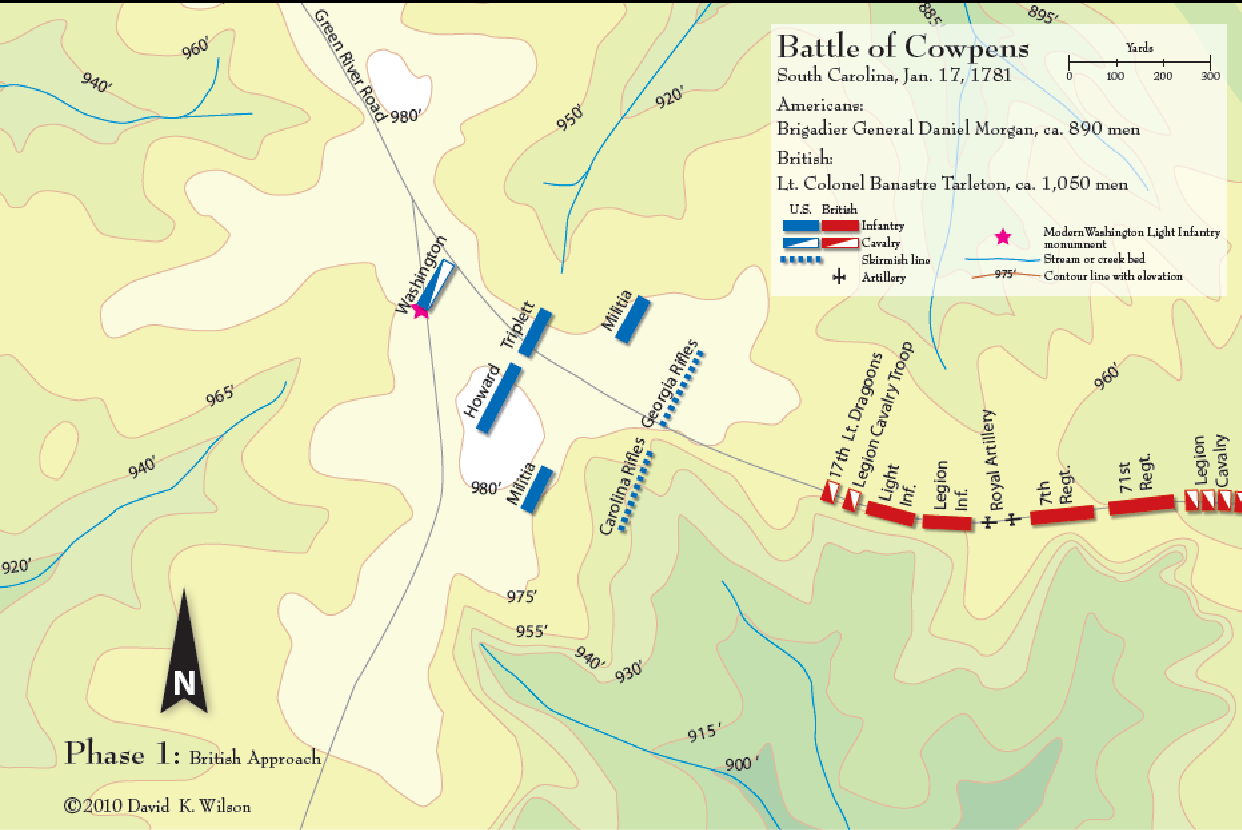
\includegraphics[width=6in]{gfx/futch1}
    \end{center}
    \caption{Terrain overview of the Battle of Cowpens. \cite{wilson_blogmap}}
    \label{terrain1}
\end{figure}

The landscape at Cowpens, given current advances in tactics and technology,
would be considered a ``killing ground'' or optimal ambush point.  Considering
the equipment and combat tactics of the time, it was a perfectly suited
battleground for the forces involved.  Tarleton considered it ``An open meadow
(for cattle grazing) about 500 yards deep and the same wide, gently undulating,
not much in the way of trees and undergrowth; good terrain to maneuver
infantry; good space to use cavalry once the enemy was broken.  The Mill Gap
road bisected the field North to South'' \cite[326]{stephenson_patriot_2007}.
From Morgan's perspective the landscape was ``relatively flat open ground
sparsely scattered with red oak and pine, the site was ideal for grazing cows
or fighting European style battles.  From the direction the British must come
(Northwest along Mill Gap Road), a single trail opened into a narrow plain that
sloped gently but unevenly uphill to the center of the pens''
\cite[45]{moncure_cowpens_1996}.  The only avenue of approach for the British
was the Mill Gap Road, a trail that had become extremely muddy due to recent
rains in the region. ``The advance of the British in the dark across a country
cut by ravines and swollen, muddy creeks was slow''
\cite[126]{lumpkin_savannah_1981}.  The topographic map below
\cite{wilson_blogmap} shows the terrain surrounding the battle site.  

Morgan, in seizing what limited high ground there was, had the advantage of
Tarleton in regards to observation during the British infiltration, but any
benefit was negated during the battle due to the gently sloping terrain once
Tarleton's forces had entered the meadow.  The British's indirect fire weapons
were not influenced by the terrain at all. 

For a relatively small battlefield, there was a great deal of important or key
terrain to be had.  One of the primary ones was a series of crests near the
center of the field: ``They found a slope lightly forested in hardwoods and
pine, possibly 150 yards long. This rose to a low ridge, dipped down to a
shallow swale, and rose again to a higher ridge.  Just behind the crown of the
second ridge was a deeper gully in which cavalry might be concealed.  The depth
of the second draw was such that horsemen could rise and their stirrups and see
all the way down the slope to the forest from which the British must come''
\cite[126]{lumpkin_savannah_1981}. This saddle in between two crests was the
perfect depth to both shield cavalry from attacking forces and to allow them
visibility of the battle with little effort.   Another piece of key terrain was
the marshland that braced both sides (east and west) of the Continental line.
``The flanks were close to the marshy ground of two creeks that bracketed the
Cowpens'' \cite[327]{stephenson_patriot_2007}.  The marsh on both sides of the
battlefield created a canalization effect for the attacking British, limiting
their ability to flank the Continental forces.  

Operationally, the terrain had a different impact for each side; Morgan used
the gully to obscure his cavalry and the marshes on either side of his forces
to limit the possibility of an enemy flank, But Tarleton appears to have
disregarded those factors and did not account for their impact during the
battle.  ``Morgan noted the way the land fell off to the left and right toward
several creeks.  The Cowpens was bordered by marshy ground that would make it
difficult for Tarleton to execute any sweeping flank movements with his
cavalry'' \cite[45]{fleming_cowpens_1988}.

The aforementioned marshes were a key obstacle in the fight, hemming and
canalizing the British into fighting straight on and limiting any flanking
movements.  That being said, the area in which the majority of the fighting
took place in was ``an open rolling woodland of first-growth pines and
hardwoods, excellent country for cavalrymen but with very little cover for
riflemen'' \cite[124]{lumpkin_savannah_1981}.  The terrain definitely
influenced the battle, it allowed Morgan to anchor his forces to the low hill
in the center and tie them into the edge of a marsh on the eastern side of the
battleground, and it led Tarleton to make an assumption that this fight was
going to be fought the way he was accustomed to: ``the ground was optimal for
Tarleton's cavalry, as the British commander noted, although it sloped gently
upward toward the American forces'' \cite[46]{moncure_cowpens_1996}.

Given the nature of the terrain and the style of warfare at the time, there was
not much in the way of cover or concealment to be had.  In fact, ``all sources
agree the battlefield was partially open with `not one single bush on the field
of battle to entangle the troops.'''\cite[66]{babits_devil_2001}. That being
said, Morgan made excellent use of the dip in elevation behind his troops:
``Behind the main line, in a shallow gully, Morgan parked William Washington's
3rd Continental Light Dragoons (82 men) together with 45 volunteer horsemen
drawn from the militia'' \cite[327]{stephenson_patriot_2007}.  The lack of
cover or concealment clearly led Tarleton to believe that this fight would be
on his terms and fought in a manner in which he was familiar.  


\paragraph{Observation and Fields of Fire}

\ldots

\paragraph{Avenues of Approach}

\ldots

\paragraph{Key Terrain}

\ldots

\paragraph{Obstacles}

\ldots

\paragraph{Cover and Concealment}

\ldots

\subsection{Comparison of Opposing Forces}

\ldots

\subsubsection{Strength and Composition}

\ldots

\subsubsection{Weapsons Technology}

\ldots

\subsubsection{Sustainment and Logistics}

\ldots

\subsubsection{Health Service Support}

\ldots

\subsubsection{Command, Control, and Communications}

\ldots

\subsubsection{Intelligence}

\ldots

\subsubsection{Information Operations}

\ldots

\subsubsection{Tactical Doctrine and Training}

\ldots

\subsubsection{Condition and morale}

\ldots

\subsubsection{Civil Affairs}

\ldots

\subsubsection{Law of War / Enemy Prisoners of War}

\ldots

\subsubsection{Leadership}

\ldots

\subsection{Feasible Courses of Action}

The tactical courses of action for both the Continentals and British were in
many ways dictated by customs and knowledge of tactics of the era.  Morgan,
performing a tactical retrograde away from Tarleton toward the broad river, was
limited in his options.  He could fight a battle against the British, continue
moving toward the river and hope to stay ahead of them, or use his forces to
harass the enemy without becoming decisively engaged.  Morgan chose the first
option, ``with the broad river behind and to the east of his force, he chose to
face Tarleton.  Morgan chose his ground wisely.  He anchored his defense on a
low hill and arrayed his infantry to the south'' \cite[32]{brinkley_back_1998}.

Once that choice was made, Morgan ran into a completely different problem: how
was he to array his forces to face the British?  He had the option of sticking
to tradition, but he had noticed that ``repeatedly in earlier battles,
inexperienced militia had ruined everything for the Revolutionaries by fleeing
the field'' \cite[30]{weigley_partisan_1970}.  That being the case, he chose
instead to ``deploy progressively stronger infantry to shoot up the British as
they advanced'' \cite[71]{babits_devil_2001}.  Utilizing different types of
assets in a combined arms fight was nothing new, but Morgan added a twist: he
integrated the militia's tendency to run away into his plan, and used it to his
benefit.

Tarleton's choices were similarly dictated by current techniques of battle, as
well as by the necessity to react to Morgan's activities.  The broad choices he
had were to hound the Revolutionaries and force a confrontation, or to forego
the chase and lay an ambush in a place of his choosing.  Tarleton chose to
``hang upon General Morgan's rear to cut off any militia reinforcements that
might show up'' \cite[46]{fleming_cowpens_1988}.  He hoped to catch Morgan as
his forces were crossing the Broad River and claim a complete victory against
the American forces.  On the smaller, tactical scale, the British commander
chose to form up as custom and tradition demanded upon the battlefield:  ``as
Tarleton had done in the past, he sent the legion cavalry to disperse the
militia and gain information of Morgan's dispositions''
\cite[33]{brinkley_back_1998}.

In respect to understanding the complete situation, Morgan had a much greater
feel for the terrain, friendly forces, and enemy forces than Tarleton did.  He
adjusted his tactics to compensate for the propensity of the Militia to cut and
run when pressed: ``therefore, Morgan in an act of shear (sic) genius, arrayed
his militia in the first rank with a line of forward skirmishers.  His
Continentals constituted the third rank.  Morgan's orders to the militia were
simple and clear: fire two or three well aimed shots then move to the rear and
flanks as a reserve'' \cite[32]{brinkley_back_1998}. Tarleton, though he did
have a good understanding of the terrain, did not see any need to adjust his
tactics as they had always served him well, and proceeded to face his opponent
with standard battle lines.  This attitude was enforced by Morgan: ``Morgan's
trap depended on breaking down the British, and, if Tarleton could not see the
American lines, the later appearance of new, stronger lines would come as
something of a surprise'' \cite[82]{babits_devil_2001}.  The limited visibility
of the morning and inability for a full reconnaissance kept the fact that
Morgan interspersed his militia with skirmishers from the British, and did not
allow Tarleton  a full understanding of the battle that was about to commence.

\subsection{Tactical Missions of the Antagonists}

Morgan had been given a great deal of leeway in his mission from higher, he was
given ``orders to conduct himself either offensively or defensively, as your
own prudence and discretion may direct -- acting with caution and avoiding
surprises by every possible precaution'' \cite[27]{weigley_partisan_1970}.
Tarleton's orders were to ``pursue Morgan and either destroy him or force him
to retreat over the Broad River again'' \cite[30]{fleming_cowpens_1988}. Based
upon his chosen course of action, Morgan's likely tactical missions were to
occupy the key terrain in the area, secure his troops, then canalize and
destroy the British forces.  Tarleton's mission set would have included
attacking by fire to defeat enemy forces and neutralize their capability for a
counterattack or to conduct follow on operations.  Both the Continental and
British Commanders' tactical missions were consistent with the orders they
received from their superiors.
